
The closed loop block diagram including an integrator is shown in Figure~\ref{fig:hw_mass_PID_root_locus}.
\begin{figure}[htbp]
   \centering
   %\includegraphics[width=0.6\textwidth]{6_design_studies/figures/hw_mass_PID_root_locus.pdf}
   \ifsolutionmanual
   
   \includegraphics[width=0.6\textwidth]{6_design_studies/figures/hw_mass_PID_root_locus.pdf}
   
   \else
   \includegraphics[width=0.6\textwidth]{../../../../6_design_studies/figures/hw_mass_PID_root_locus.pdf}

   
   \fi
   \caption{PID control for the mass spring damper.}
   \label{fig:hw_mass_PID_root_locus}
\end{figure}
The characteristic equation is given by
\[
1+P(s)C(s) = 1+\left(\frac{\frac{1}{m}}{s^2+\frac{b}{m}s+\frac{k}{m}}\right)\left(\frac{k_Ds^2+k_Ps+k_I}{s}\right) = 0.
\]
Multiplying by the denominator and simplifying gives
\[
s^3+\left(\frac{b+k_K}{m}\right)s^2 + \left(\frac{k+K_P}{m}\right)s + \frac{k_I}{m} = 0.
\]
In Evan's form we have
\[
1 + k_I\left(\frac{\frac{1}{m}}{s^3 + \left(\frac{b+k_D}{m}\right)s^2 + \frac{k+k_P}{m}s}\right) = 0.
\]
The appropriate Matlab command is therefore
\begin{lstlisting}
>> L = tf([1/m],[1, (b+kd)/m, (k+kp)/m,0]);
>> figure(1), clf, rlocus(L);
\end{lstlisting}
